% !TeX spellcheck = en_GB

\section{Extension Toward a Model of Eyeblink Conditioning}
\label{sec:cerebellum_eyeblink}

Given the above model for the Golgi and granule cells, we can now introduce learning into the model to test the behaviour of the system in an eyeblink conditioning task.
Since we are mostly interested in whether it is possible at all to decode functions online from the Granule cell activities, we do not focus on biological detail for the added components beyond the standard \NEF techniques discussed in \Cref{sec:nef}.
For example, we do not account for Dale's principle for the added neuron populations and use relatively few spiking neurons at high maximum firing rates (\SIrange{200}{400}{\per\second}) to represent individual ensembles.

\subsubsection{Network description and learning}
Our final network architecture is depicted in \Cref{fig:eyeblink_network}.
Consistent with the adaptive-filter hypothesis of cerebellar function and as discussed in \Cref{sec:cerebellum_microcircuit}, we assume that the error signal $\varepsilon(t)$ originates from the inferior olive (\IO).
This signal is the difference between the conditioned response (what the model has learned so far), and the unconditioned response (the motor response produced by the innate eyeblink reflex).
We model the eyelid as a first-order dynamical system that receives a velocity command.
The reflexive velocity command has been fitted to the \UR data in \citet{heiney2014cerebellardependent}.

\begin{figure}
	\centering%
	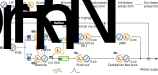
\includegraphics{media/chapters/05_cerebellum/eyeblink_network.pdf}
	\caption[Overview of the final eyeblink conditioning network]{Overview of the final eyeblink conditioning network. Note that our model of the Purkinje cells and the deep cerebellar nuclei is less biologically detailed than the Granule-Golgi circuit.
	}
	\label{fig:eyeblink_network}
\end{figure}

To adjust the connection weights between the granule cells and the Purkinje cells, we use the Prescribed Error Sensitivity (\PES) rule defined by \citet{macneil2011finetuning}, a biologically plausible variant of the classic delta learning rule.
Let $w^{\mathrm{Gr}\to\mathrm{Pu}}_{ij}$ be the connection weight between the $j$th granule cell and the $i$th Purkinje cell, $\eta$ a learning rate parameter, $a^\mathrm{Gr}_j(t)$ the $j$th post-synaptic granule cell activity filtered by a low-pass filter with time-constant $\tau_\mathrm{learn}$, and $e^\mathrm{Pu}_i \in \{-1, 1\}$ the encoder of the $i$th Purkinje cell.
The \PES learning rule is given as
\begin{align*}
	\frac{\partial}{\partial t} w^{\mathrm{Gr}\to\mathrm{Pu}}_{ij}(t) &= -\eta \varepsilon(t) e^\mathrm{Pu}_i a^\mathrm{Gr}_j(t) = -\eta \sum_{k} w^{\mathrm{IO}\to\mathrm{Pu}}_{ik} a^\mathrm{IO}_k(t) \,,
\end{align*}
where $a^\mathrm{IO}_k(t)$ is the activity of the $k$th \IO cell, and $w^{\mathrm{IO}\to\mathrm{Pu}}_{ik}$ are the synaptic weights between the $k$th \IO cell and the $i$th Purkinje cell.
These weights are the product of the Purkinje cell encoder $e_i^\mathrm{Pu}$ and a decoding vector $\vec d_k^\mathrm{IO}$ that linearly decodes the error signal $\varepsilon(t)$ from \IO cell activity.

Most parameters were set based on biological data; the synaptic time-constant $\tau = \SI{5}{\milli\second}$ except in the Granule-Golgi microcircuit, as described above.
The only free parameters are the learning rate $\eta=180\times 10^{-6}$, $\tau_\mathrm{pRN} = \SI{100}{\milli\second}$ for the connections involving the pRN, and $\tau_\mathrm{learn} = \SI{60}{\milli\second}$ for filtering the granule cell activity in the learning rule.
The learning rate was adjusted to match the number of trials typically needed for mice to learn the task ($\approx 300$ trials).
Velocity commands smaller than $v_\mathrm{th} = \SI{2}{\milli\metre\per\second}$ are counted as zero.

\begin{figure}
	\centering%
	\includegraphics{media/chapters/05_cerebellum/blink_trials_panel.pdf}
	\caption[Model and experimental data for the eyeblink conditioning task]{Model and experimental data for the eyeblink conditioning task. \textbf{(A, B)} Maximum \CR triggered eyelid closure over $500$ trials for six random instances of the model/experimental animals. Gray dots correspond to the eyelid closure at the time of the \US. Black line is the moving average over 11 trials. Blue dotted lines correspond to an experimental day, that is, $100$ trials in simulation, and up to $100$ trials in the animal experiment. \textbf{(C, D)} Eyelid closure trajectory averaged over one experimental day and all six models/animals. \textbf{(E)} Eyelid velocity signal decoded at the Purkinje cells compared to the reflex-triggered velocity signal. Data for \textbf{(B, D)} adapted from \protect\citet{heiney2014cerebellardependent}.}
	\label{fig:result-basic}
\end{figure}

\subsubsection{Results}
\Cref{fig:result-basic} shows the behaviour of a typical run of the detailed version of our model performing the eyeblink conditioning task over 500 trials.
The \enquote{tone} (\CS) is modelled as a rectangle pulse with $t_\mathrm{on} = \SI{100}{\milli\second}$.
The \enquote{puff} (\US) occurs \SI{250}{\milli\second} after the \CS onset.
The model learns to have the eye closed when the puff occurs. Notably, individual instances of the network show slight differences in learning speed, just as individual experimental animals do.

While our model reproduces key features of eyeblink conditioning, its behaviour differs from the experimental data in some aspects.
Foremost, the model does not reproduce the increase in learning speed over time; to the contrary, learning slows down as the model converges to the optimal set of parameters.
Furthermore, our model shows far less inter-trial variance compared to experimental animals.
We think that the reasons for this are twofold.
First, the $10\,000$ granule cells used in our experiments provide an on average very stable temporal basis from which we can decode the motor control signal.
Second, we do not model external systems that might interfere with the cerebellar motor commands, such as signals originating from motor cortex, or the physics of the eyelid itself.
Since these processes may be a significant source of inter-trial variance, it is not unsurprising that our model produces a relatively noise-free output.
Still, more research in these areas will be required in the future.


\subsubsection{Discussion of the synaptic filter $\tau_\mathrm{learn}$}
The low-pass filter $\tau_\mathrm{learn}$ on the learning connection can be interpreted as summarising temporal filtering corresponding to the mechanisms driving synaptic plasticity \citep[e.g.,][Chapter~66]{kandel2012principles}.
Functionally, $\tau_\mathrm{learn}$ is required to reproduce the observation that the animal will close the eye \emph{before} the puff occurs as learning progresses.
Without the filter, the system learns to close the eye soon \emph{after} the puff; our system tries to exactly re-create the motor pattern produced by the unconditioned reflex---which closes the eye \emph{after} the puff happens.

However, by slowing the passage of information from the Cerebellar Nucleus back to the \IO, we are effectively comparing the reflex at one point in time to the generated output from the cerebellum at an \emph{earlier} point in time.
This allows the new learned reflex to occur slightly earlier than the unconditioned response, and thus the eye closes before the air puff.
We note that this is a situation where adding biological detail (the synaptic filtering) improves the performance of the model.
If the model were to learn to \textit{exactly} reproduce the \UR given the \CS, then the eyeblink would occur \textit{after} the puff of air, which would be a less useful response.
